
\chapter{Kramer Rate Theory}\label{kramer}
\lhead[\fancyplain{}{\bfseries\thepage}]{\fancyplain{}{\bfseries\rightmark}}
In this Chapter we make a briefly introduction in stochastic process and in Kramer Rate Theory.
\section{Fokker-Planck equation}
Fokker-Planck equation is a second order parabolic partial differential equation, and it's born during the investigation of the Brownian motion in a radiation field by Fokker and Planck \cite{K50}. This equation describe the time evolution of a probability distribution $\rho(x,t)$ in a stochastic process.
In one dimension, the Fokker-Planck equation (FPE) takes the simple form:
\begin{equation}
\frac{\partial \rho(x,t)}{\partial t} = -\frac{\partial}{\partial x} \biggl(A(x,t) \rho(x,t)\biggr) + \frac{1}{2} \frac{\partial ^2}{\partial x^2} \biggl(B(x,t) \rho(x,t) \biggr)
\label{eq:FP}
\end{equation}
with the initial condition:
\begin{equation}
\rho(x,t_0|x_0,t_0) = \delta(x-x_0)
\end{equation}
The first term in the equation ~\ref{eq:FP} is the drift equation, while the last term is the diffusion equation.
Every stochastic process described by a conditional probability satisfying the FPE is equavalent to the Ito stochastic differential equation (SDE)
\begin{equation}
dx(t) = A(x(t),t)dt + \sqrt{B(x(t),t)} dw_t
\end{equation}
and the two descriptions are complementary to each other.


\section{Bistability and Escape Problems}
In Nature exist some systems which have at least two possible stable states. This kind of systems are known as \emph{bistable systems} \cite{K50}. For such systems there are some problems of interest:
\begin{itemize}
\item How stable are the various states relative to each other?
\item How long does it take for a system to switch spontaneously from one state to onother?
\item How is the path in the relevant state space?
\item How does a system relax from an unstable state?
\end{itemize}
These questions can all be answered reasily for one-dimensional diffusion processes.
\subsection{Diffusion in a Double-Well Potential in one dimension}
We consider the system in which we have the probability density $\rho(x,t)$ of a prarticle, which obeys the Fokker-Planck equation:
\begin{equation}
\frac{\partial \rho}{\partial t } = \frac{\partial}{\partial x} V'(x)\rho + D \frac{\partial ^2 }{\partial x^2} \rho
\end{equation}
The shape of $V(x)$ is shown in Figure \ref{fig:kr}.
\begin{figure}[h]
\centering
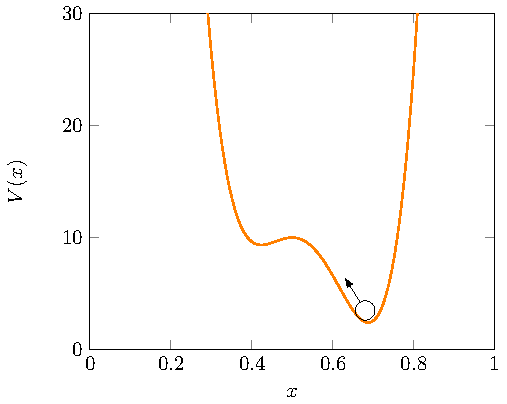
\includegraphics[scale=1.2]{images/kramerwell.pdf}
\caption{\emph{Example of double-well potential.}}
\label{fig:kr}
\end{figure}

There are two minima at $a$ and $c$ and in between, a local maximum $b$. The stationary distribution is
\begin{equation}
\rho_s(x) = \mathcal{N} e^{-\frac{V(x)}{D}}
\end{equation}
where $\mathcal{N}$ is the normalization constant.This distribution explains the bistability of the system, since, we have two local maxima of the potential in $a$ and $c$. (see Figure \ref{fig:kramerpot}).

\begin{figure}[h]
\centering
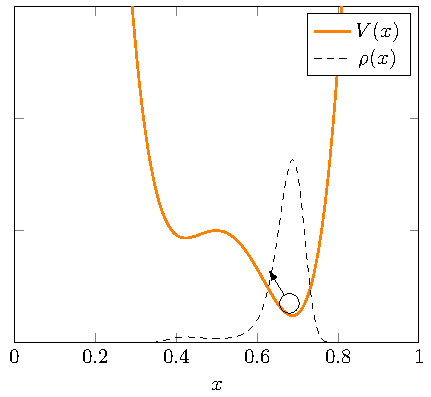
\includegraphics[scale=1.2]{images/kramerpot.pdf}
\caption{\emph{The distribution (dashed) explains the bistability of the system, since, we have two local maxima of the potential in $a$ and $c$..}}
\label{fig:kramerpot}
\end{figure}

\subsection{Behaviour for $D=0$}
In this case, $x(t)$ obeys the differential equation
\begin{equation}
\frac{dx}{dt} = - V'(x)
\end{equation}
with initial condition $x(0) = x_0$.
Now, since
$$
\frac{dV(x)}{dt} = V'(x)\frac{dx}{dt} = - (V'(x))^2 < 0 
$$

$x(t)$ always moves in such a way as to minimise $V(x)$, and stops only when $V'(x)$ is zero. Thus, depending on whether $x_0$ is grater than or less than $b$, the particle ends up at $c$ or $a$, respectively. Once the particle is at $a$ or $c$, it stays there. If it starts exactly at $b$, it also stay there, thoug the slightest perturbation drives it to $a$ or $c$. Thus, $b$ in an \emph{unstable} stationart point and $a$ and $c$ are stable.
\subsection{Behaviour if $D$ is small}
With the addition of noise, the situation changes. The stationary state can be approximated asymptotically as folows. Assuming $V(x)$ is everywhere sufficiently smooth, we can write
\begin{equation}
\begin{split}
V(x) & \simeq V(a) + \frac{1}{2} V''(a)(x-a)^2 \\
& \simeq V(c) + \frac{1}{2} V''(c)(x-c)^2 
\end{split}
\end{equation}
for $|x-a|$ and $|x-c|$ small, respectively.
If $D$ is very small, then we may approximate
\begin{equation}
\begin{split}
\rho_s(x)  &\simeq \mathcal{N} \exp\biggl(-\frac{V(a)}{D} - \frac{1}{2} V''(a)\frac{(x-a)^2}{D}\biggr) \\
&\simeq \mathcal{N} \exp\biggl(-\frac{V(c)}{D} - \frac{1}{2} V''(c)\frac{(x-c)^2}{D}\biggr) 
\end{split}
\label{eq:r}
\end{equation}
And zero elsewhere.
So that:
\begin{equation}
\mathcal{N}^{-1}  \simeq e^{-\frac{V(a)}{D}} \sqrt{\frac{ 2 \pi D }{V''(a)}} + e^{-\frac{V(c)}{D}} \sqrt{\frac{ 2 \pi D }{V''(c)}}
\end{equation}
Now suppose as in drawn in Figure \ref{fig:kramerpot} 
$$
V(a)>V(c)
$$
Then for small enough $D$, the second term is larger than the first and $\mathcal{N}^{-1}$ can be approximated by it alone. So, substituing into ~\ref{eq:r} we find
\begin{equation}
\rho_s(x) = \sqrt{\frac{V''(c)}{2 \pi D}} \exp\biggl(-\frac{1}{2}V''(c)\frac{(x-c)^2}{D}\biggr)
\end{equation}
for 
$$
|x-c| \sim \sqrt{D}
$$
and zero otherwise.
This means that in the limit of very small $D$, the deterministic stationary state at which $V(x)$ has an absolute minimum is the more stable state in the sense that in the stochastic stationary state, $\rho_s(x)$ is very small everywhere except in its immediate vicinity. This means, differently from the previous results, that due to the noise the  equilibrium points $a$ and $c$ are no longer equally stable.







\section{Kramer Rate Theory}
We consider the Smoluchowski equation:
\begin{equation}
dx = -V'(x)dt + \sqrt{2T} dw_t
\end{equation}

\begin{figure}
\centering
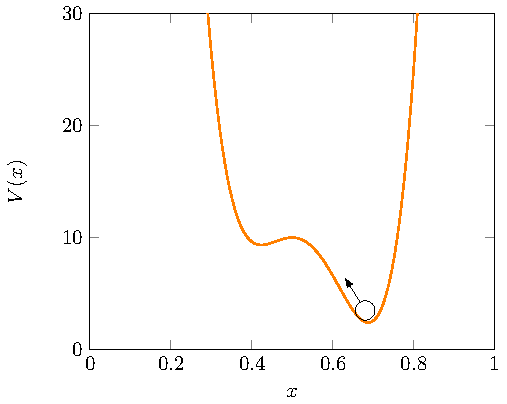
\includegraphics[scale=1.2]{images/kramerwell.pdf}
\caption{\emph{Example of double-well potential.}}
\label{fig:kr}
\end{figure}


where $V(x)$ is a double well potential with $x_a$ and $x_c$ local minima separated by a saddle point $x_b$: To compute the transition probability from the left well to the right well we consider the stationary solution of the Fokker-Planck equation:
\begin{equation}
\frac{\partial \rho}{\partial t } = \frac{\partial}{\partial x} V'(x)\rho + T \frac{\partial ^2 }{\partial x^2} \rho
\end{equation}

with the boundary condition that we have a source in the point $x_{-} < x_a$ and an absorbing boundary at the point $x_{+} > x_c$. We assume that the temperature $T$ is much les of the potential barrier $V_b - V_a$ and we look for a solution that reduces to the form:
$$
e^{-\frac{V(x)}{T}}
$$
in the vicinity of the point $x_a$ that vanishes at the absorbing barrier and gives a constant current $J$ between the two wells. Let
\begin{equation}
\rho(x)=C(x)e^{-\frac{V(x)}{T}}
\end{equation}
and the particle density current $-J=V'(x)\rho + \frac{\partial \rho}{\partial x}T$ reads
$$
V'(x)C(x)e^{-\frac{V}{T}} + C'(x)Te^{-\frac{V}{T}} - V'(x)C(x)e^{-\frac{V}{T}} = -J
$$
so that: 
$$
C'(x) = -\frac{J}{T}e^{\frac{V}{T}}
$$
and we integrate with the condition $C(x_{+}) = 0$:
$$
C(x) = \frac{J}{T}\int_{x}^{x_{+}} e^{\frac{V(y)}{T}}dy
$$

The distribution reads:
$$
\rho(x) = \frac{J}{T} e^{-\frac{V(x)}{T}}\int_x^{x_{+}}e^{\frac{V(y)}{T}}dy.
$$

When$x \simeq x_a$ the integral
$$
\int_x^{x_{+}}e^{\frac{V(y)}{T}}dy
$$
is stationary since $V'(x_a) = 0$ and $\rho(x)$ has the behavior of $e^{-\frac{V(x)}{T}}$.
Then we have to compute the number of particles $n_a$ in the left well
$$
n_a = \frac{J}{T}\int_{-\infty}^{x_{b}} e^{-\frac{V(x)}{T}} \int_{x}^{x_+} e^{\frac{V(y)}{T}} dy dx
$$

We approximate the integrals using the saddle point method:
$$
e^{\frac{V(y)}{T}} \simeq e^{\frac{V_b}{T} - \frac{\omega^2_b}{2T}(y-x_b)^2}
$$
$$
e^{\frac{V(x)}{T}} \simeq e^{\frac{V_a}{T} - \frac{\omega^2_a}{2T}(x-x_a)^2}
$$

so we compute:
$$
\frac{n_a}{J} = \frac{1}{T} e^{\frac{V_b-V_a}{T}}\int_{-\infty}^{x_b}dxe^{-\frac{\omega_a^2}{2T}(x-x_a)^2}\int_x^{x_+}e^{-\frac{\omega_b^2}{2T}(y-x_b)^2 }dy
$$
Then we can extend both the integrals between $-\infty$ and $+\infty$:
$$
\int_{-\infty}^{+\infty}dxe^{-\frac{\omega_a^2}{2}(x-x_a)^2} = \frac{\sqrt{2 \pi T}}{\omega_a}\frac{n_a}{J}=\frac{2\pi}{\omega_a\omega_b}e^{\frac{V_b-V_a}{T}}
$$
And we find the transition probability rate:
$$
k_{a\to c} = \frac{J}{n_a} \simeq \frac{\omega_a \omega_b}{2 \pi} e^{\frac{V_b-V_a}{T}}
$$

The fact that $k_c$ does not depend on $x$ is due to the fast relaxation scale time inside the potential well with respect to the escape time scale from the potential well and to the quasi-stationary distribution that concentrates the particles near the local minimal point where the effect of the potential can be approximated by a parabolic potential.
In this systems the transition probability $k_c$ can be used to estimate the potential.
In Chapter \ref{analysis} we try to estimate $k_c$ for Boolean Networks.
